
%% LyX 2.2.1 created this file.  For more info, see http://www.lyx.org/.
%% Do not edit unless you really know what you are doing.
\documentclass{article}\usepackage[]{graphicx}\usepackage[]{color}
% maxwidth is the original width if it is less than linewidth
% otherwise use linewidth (to make sure the graphics do not exceed the margin)
\makeatletter
\def\maxwidth{ %
  \ifdim\Gin@nat@width>\linewidth
    \linewidth
  \else
    \Gin@nat@width
  \fi
}
\makeatother

\definecolor{fgcolor}{rgb}{0.345, 0.345, 0.345}
\newcommand{\hlnum}[1]{\textcolor[rgb]{0.686,0.059,0.569}{#1}}%
\newcommand{\hlstr}[1]{\textcolor[rgb]{0.192,0.494,0.8}{#1}}%
\newcommand{\hlcom}[1]{\textcolor[rgb]{0.678,0.584,0.686}{\textit{#1}}}%
\newcommand{\hlopt}[1]{\textcolor[rgb]{0,0,0}{#1}}%
\newcommand{\hlstd}[1]{\textcolor[rgb]{0.345,0.345,0.345}{#1}}%
\newcommand{\hlkwa}[1]{\textcolor[rgb]{0.161,0.373,0.58}{\textbf{#1}}}%
\newcommand{\hlkwb}[1]{\textcolor[rgb]{0.69,0.353,0.396}{#1}}%
\newcommand{\hlkwc}[1]{\textcolor[rgb]{0.333,0.667,0.333}{#1}}%
\newcommand{\hlkwd}[1]{\textcolor[rgb]{0.737,0.353,0.396}{\textbf{#1}}}%
\let\hlipl\hlkwb

\usepackage{framed}
\makeatletter
\newenvironment{kframe}{%
 \def\at@end@of@kframe{}%
 \ifinner\ifhmode%
  \def\at@end@of@kframe{\end{minipage}}%
  \begin{minipage}{\columnwidth}%
 \fi\fi%
 \def\FrameCommand##1{\hskip\@totalleftmargin \hskip-\fboxsep
 \colorbox{shadecolor}{##1}\hskip-\fboxsep
     % There is no \\@totalrightmargin, so:
     \hskip-\linewidth \hskip-\@totalleftmargin \hskip\columnwidth}%
 \MakeFramed {\advance\hsize-\width
   \@totalleftmargin\z@ \linewidth\hsize
   \@setminipage}}%
 {\par\unskip\endMakeFramed%
 \at@end@of@kframe}
\makeatother

\definecolor{shadecolor}{rgb}{.97, .97, .97}
\definecolor{messagecolor}{rgb}{0, 0, 0}
\definecolor{warningcolor}{rgb}{1, 0, 1}
\definecolor{errorcolor}{rgb}{1, 0, 0}
\newenvironment{knitrout}{}{} % an empty environment to be redefined in TeX

\usepackage{alltt}

\usepackage{geometry}
\geometry{verbose,tmargin=2.5cm,bmargin=2.5cm,lmargin=2.5cm,rmargin=2.5cm}
\IfFileExists{upquote.sty}{\usepackage{upquote}}{}
\begin{document}


\title{Code: ACG, CGU}

\author{GCATR Tool}

\maketitle

\begin{knitrout}
\definecolor{shadecolor}{rgb}{0.969, 0.969, 0.969}\color{fgcolor}\begin{kframe}
\begin{alltt}
\hlstd{is_code} \hlkwb{=} \hlkwd{code_check_if_code}\hlstd{(params}\hlopt{$}\hlstd{code)}
\hlstd{cn_circular} \hlkwb{<-} \hlkwd{code_check_if_cn_circular}\hlstd{(params}\hlopt{$}\hlstd{code)}
\hlstd{circular} \hlkwb{<-} \hlkwd{code_check_if_circular}\hlstd{(params}\hlopt{$}\hlstd{code)}

\hlstd{comma_free} \hlkwb{<-} \hlkwd{code_check_if_comma_free}\hlstd{(params}\hlopt{$}\hlstd{code)}
\hlstd{self_comp} \hlkwb{<-} \hlkwd{code_check_if_self_complementary}\hlstd{(params}\hlopt{$}\hlstd{code)}
\hlstd{acid} \hlkwb{<-} \hlkwd{code_get_acid}\hlstd{(params}\hlopt{$}\hlstd{code)}
\end{alltt}
\end{kframe}
\end{knitrout}



\section{Prperties}
\begin{itemize}
	\item acid: RNA
Tuple length $\ell$ = 3 \item Circular:  TRUE 
 \item Comma-Free:  TRUE 
 \item $C_\ell$ Circular:  TRUE 
 \item Self-Complementary:  TRUE
\end{itemize}

\begin{knitrout}
\definecolor{shadecolor}{rgb}{0.969, 0.969, 0.969}\color{fgcolor}\begin{kframe}
\begin{alltt}
\hlstd{G} \hlkwb{<-} \hlkwd{code_factor_graph}\hlstd{(params}\hlopt{$}\hlstd{code,} \hlnum{TRUE}\hlstd{,} \hlnum{TRUE}\hlstd{)}
\end{alltt}
\begin{verbatim}
## 2 - -1
\end{verbatim}
\begin{alltt}
\hlkwd{plot}\hlstd{(G)}
\end{alltt}
\end{kframe}\begin{figure}

{\centering 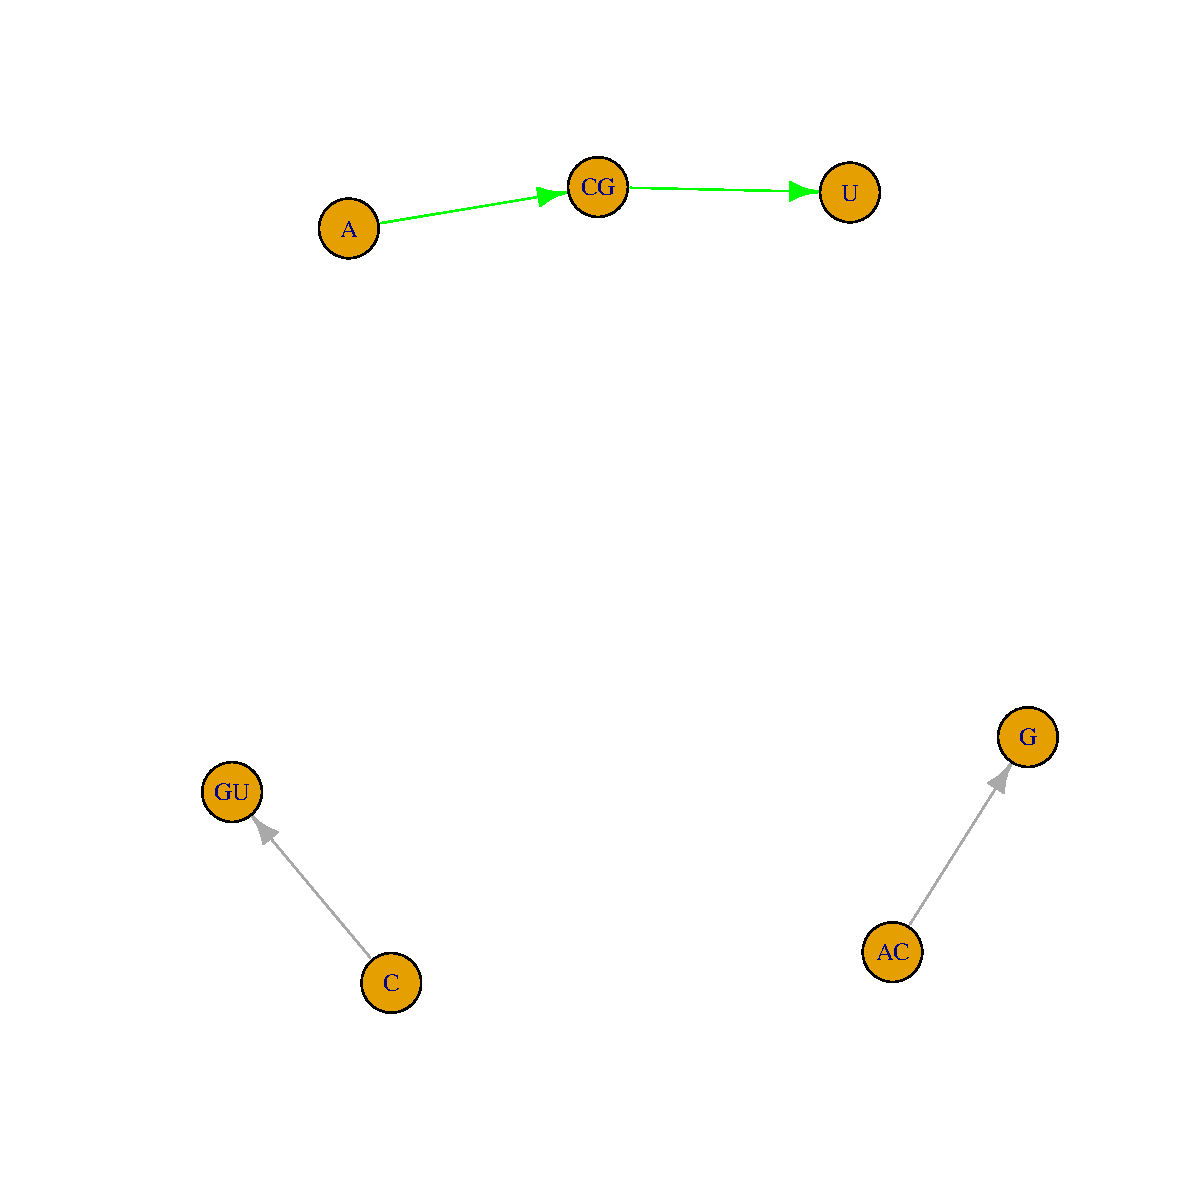
\includegraphics[width=.8\linewidth]{figure/minimal-representing-graph-1} 

}

\caption[Representing Graph]{Representing Graph}\label{fig:representing-graph}
\end{figure}


\end{knitrout}

\begin{knitrout}
\definecolor{shadecolor}{rgb}{0.969, 0.969, 0.969}\color{fgcolor}\begin{kframe}
\begin{alltt}
\hlkwa{if}\hlstd{(circular) \{}
  \hlstd{G} \hlkwb{<-} \hlkwd{code_factor_longest_path}\hlstd{(params}\hlopt{$}\hlstd{code)}
\hlstd{\}} \hlkwa{else} \hlstd{\{}
  \hlstd{G} \hlkwb{<-} \hlkwd{code_factor_cycle}\hlstd{(params}\hlopt{$}\hlstd{code)}
\hlstd{\}}
\hlkwd{plot}\hlstd{(G)}
\end{alltt}
\end{kframe}\begin{figure}

{\centering 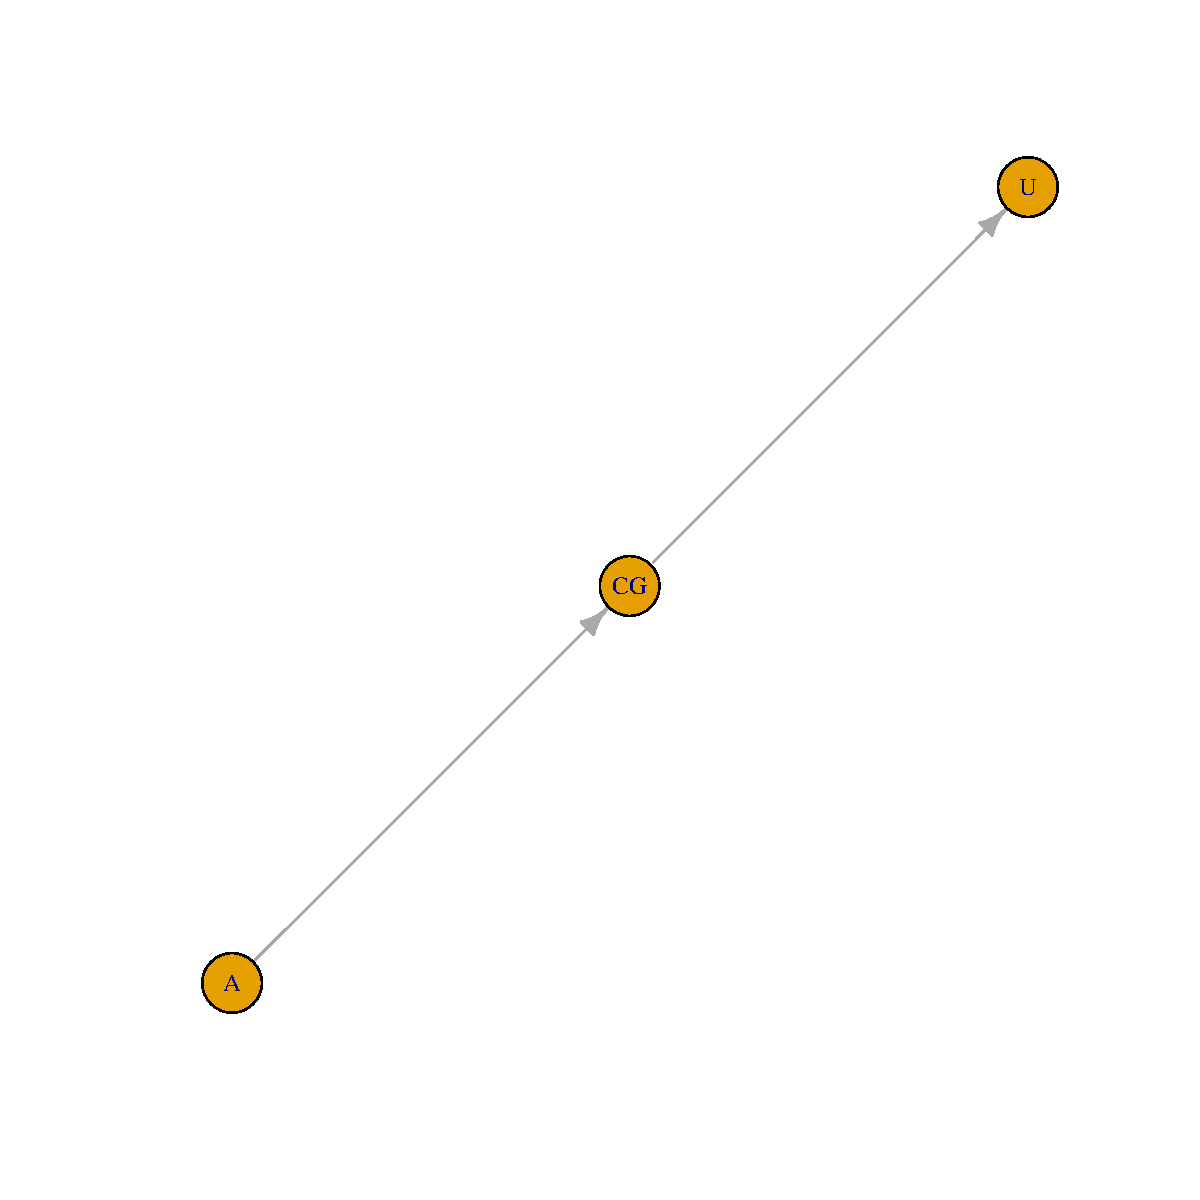
\includegraphics[width=.8\linewidth]{figure/minimal-graph-properties-1} 

}

\caption[Representing Graph longest path or cycle]{Representing Graph longest path or cycle}\label{fig:graph-properties}
\end{figure}


\end{knitrout}


% latex table generated in R 3.6.0 by xtable 1.8-4 package
% Wed Jun 26 16:00:29 2019
\begin{table}[ht]
\centering
\begin{tabular}{rllll}
  \hline
 & X\_U\_ & X\_C\_ & X\_A\_ & X\_G\_ \\ 
  \hline
U\_U & UUU - Phe & UCU - Ser & UAU - Tyr & UGU - Cys \\ 
  U\_C & UUC - Phe & UCC - Ser & UAC - Tyr & UGC - Cys \\ 
  U\_A & UUA - Leu & UCA - Ser & UAA - Stop & UGA - Stop \\ 
  U\_G & UUG - Leu & UCG - Ser & UAG - Stop & UGG - Trp \\ 
  C\_U & CUU - Leu & CCU - Pro & CAU - His & CGU - Arg \\ 
  C\_C & CUC - Leu & CCC - Pro & CAC - His & CGC - Arg \\ 
  C\_A & CUA - Leu & CCA - Pro & CAA - Gln & CGA - Arg \\ 
  C\_G & CUG - Leu & CCG - Pro & CAG - Gln & CGG - Arg \\ 
  A\_U & AUU - Ile & ACU - Thr & AAU - Asn & AGU - Ser \\ 
  A\_C & AUC - Ile & ACC - Thr & AAC - Asn & AGC - Ser \\ 
  A\_A & AUA - Ile & ACA - Thr & AAA - Lys & AGA - Arg \\ 
  A\_G & AUG - Met & ACG - Thr & AAG - Lys & AGG - Arg \\ 
  G\_U & GUU - Val & GCU - Ala & GAU - Asp & GGU - Gly \\ 
  G\_C & GUC - Val & GCC - Ala & GAC - Asp & GGC - Gly \\ 
  G\_A & GUA - Val & GCA - Ala & GAA - Glu & GGA - Gly \\ 
  G\_G & GUG - Val & GCG - Ala & GAG - Glu & GGG - Gly \\ 
   \hline
\end{tabular}
\end{table}


\end{document}
